\documentclass{beamer}
\usetheme{Madrid}
\usecolortheme{whale}

\usepackage{tikz}
\usetikzlibrary{shapes.geometric, arrows, positioning}

% Define TikZ styles
\tikzstyle{startstop} = [rectangle, rounded corners, minimum width=2.5cm, minimum height=0.8cm,text centered, draw=black, fill=red!30, font=\tiny]
\tikzstyle{process} = [rectangle, minimum width=2.5cm, minimum height=0.8cm, text centered, draw=black, fill=orange!30, font=\tiny]
\tikzstyle{decision} = [diamond, minimum width=2.5cm, minimum height=0.8cm, text centered, draw=black, fill=green!30, font=\tiny]
\tikzstyle{arrow} = [thick,->,>=stealth]

\title{SAR Narrative Generator with Audit Trail}
\subtitle{AI-Driven Compliance with Logic \& Active Learning}
\author{Team Name}
\date{\today}

\begin{document}

\frame{\titlepage}

\begin{frame}{Problem Statement}
    \begin{itemize}
        \item \textbf{High Volume, Low Efficiency}: SAR filing is manual and resource-intensive (5--6 hours per report).
        \item \textbf{Inconsistency}: Narratives vary by analyst, leading to "Defensive Reporting".
        \item \textbf{The "Black Box" Issue}: AI solutions often lack explainability, making them hard to defend to regulators.
        \item \textbf{Stagnant Models}: Existing rule-based systems generate 90\% false positives and don't learn from mistakes.
    \end{itemize}
\end{frame}

\begin{frame}{Our Solution: Dual-Engine Architecture}
    We propose an \textbf{AI-driven SAR Narrative Generator} that combines:
    \vspace{0.5cm}
    \begin{enumerate}
        \item \textbf{Quantitative Precision}: XGBoost \& Graph algorithms to detect "Needle in Haystack" anomalies.
        \item \textbf{Qualitative Context}: RAG engine retrieving \textbf{Vectorized Law} (ChromaDB) to ground the narrative.
        \item \textbf{Defensible AI}: Llama 3.1 generates narratives with \textbf{Audit Trails} (citations).
        \item \textbf{Active Learning}: A feedback loop where analyst corrections retrain the model.
    \end{enumerate}
\end{frame}

\begin{frame}{Fraud Detection Pipeline}
    \centering
    \scalebox{0.75}{
    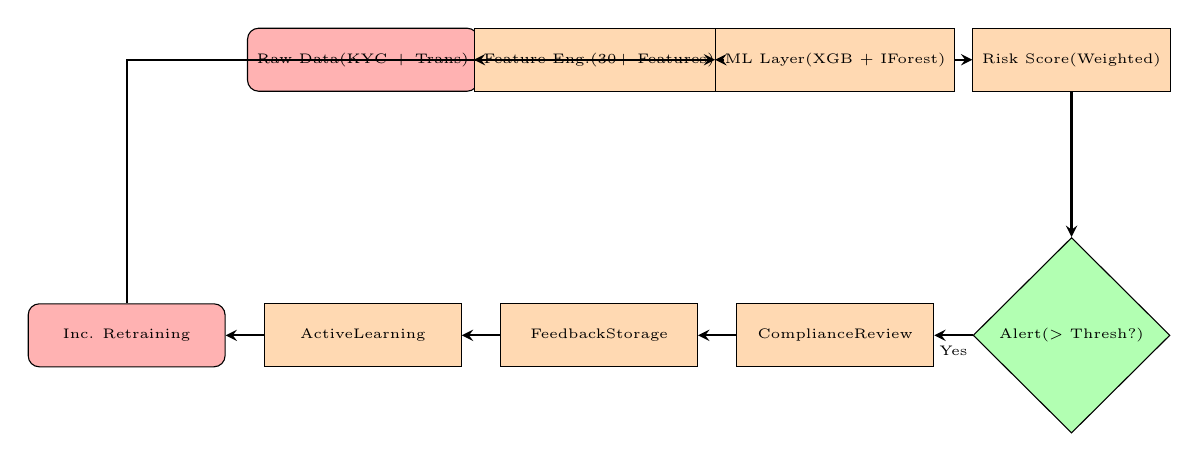
\begin{tikzpicture}[node distance=2.5cm]
        % Row 1
        \node (raw) [startstop] {Raw Data\\(KYC + Trans)};
        \node (feat) [process, right of=raw, xshift=0.5cm] {Feature Eng.\\(30+ Features)};
        \node (ml) [process, right of=feat, xshift=0.5cm] {ML Layer\\(XGB + IForest)};
        \node (score) [process, right of=ml, xshift=0.5cm] {Risk Score\\(Weighted)};
        
        % Row 2
        \node (alert) [decision, below of=score, yshift=-1.0cm] {Alert\\(> Thresh?)};
        \node (review) [process, left of=alert, xshift=-0.5cm] {Compliance\\Review};
        \node (feedback) [process, left of=review, xshift=-0.5cm] {Feedback\\Storage};
        \node (active) [process, left of=feedback, xshift=-0.5cm] {Active\\Learning};
        \node (retrain) [startstop, left of=active, xshift=-0.5cm] {Inc. Retraining};
        
        % Arrows
        \draw [arrow] (raw) -- (feat);
        \draw [arrow] (feat) -- (ml);
        \draw [arrow] (ml) -- (score);
        \draw [arrow] (score) -- (alert);
        \draw [arrow] (alert) -- node[anchor=north, font=\tiny] {Yes} (review);
        \draw [arrow] (review) -- (feedback);
        \draw [arrow] (feedback) -- (active);
        \draw [arrow] (active) -- (retrain);
        \draw [arrow] (retrain) |- (ml);
    \end{tikzpicture}
    }
\end{frame}

\begin{frame}{System Architecture}
    \begin{itemize}
        \item \textbf{Ingestion}: Kafka streaming for high-throughput transaction data.
        \item \textbf{RAG Engine}: ChromaDB stores "Golden SARs" and Regulatory Guidelines.
        \item \textbf{Generator}: Llama 3.1 (8B) fine-tuned for regulatory tone.
        \item \textbf{Audit Service}: Maps every generated claim to a source document.
        \item \textbf{Feedback Loop}: Captures "True/False Positive" labels for XGBoost retraining.
    \end{itemize}
\end{frame}

\begin{frame}{System Architecture Overview}
    \centering
    \scalebox{0.7}{
    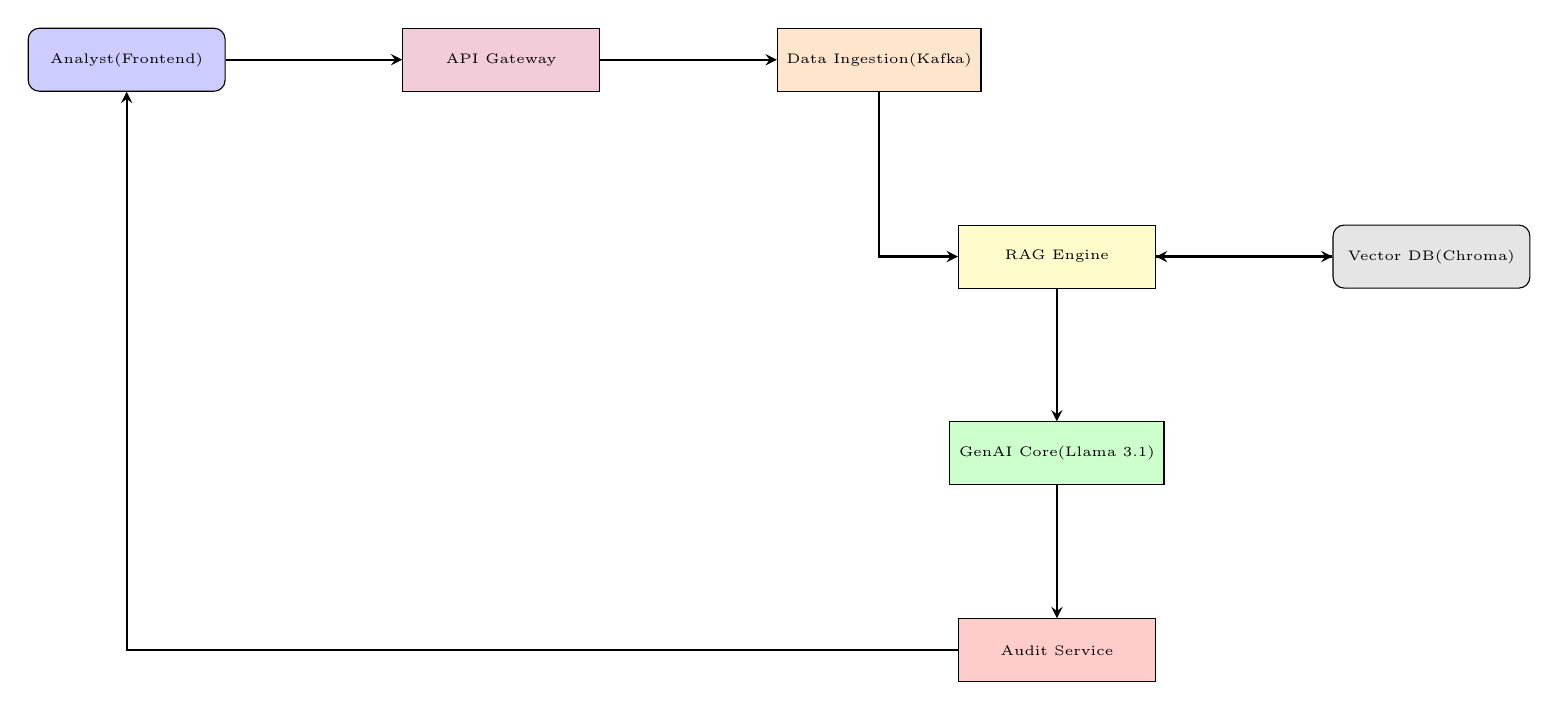
\begin{tikzpicture}[node distance=2.5cm, auto]
        % Nodes
        \node (user) [startstop, fill=blue!20] {Analyst\\(Frontend)};
        \node (api) [process, right of=user, right=1cm, fill=purple!20] {API Gateway};
        \node (kafka) [process, right of=api, right=1cm, fill=orange!20] {Data Ingestion\\(Kafka)};
        
        \node (rag) [process, below of=kafka, right=1cm, fill=yellow!20] {RAG Engine};
        \node (llm) [process, below of=rag, fill=green!20] {GenAI Core\\(Llama 3.1)};
        
        \node (vectordb) [startstop, right of=rag, right=1cm, fill=gray!20] {Vector DB\\(Chroma)};
        \node (audit) [process, below of=llm, fill=red!20] {Audit Service};
        
        % Connections
        \draw [arrow] (user) -- (api);
        \draw [arrow] (api) -- (kafka);
        \draw [arrow] (kafka) |- (rag);
        \draw [arrow] (rag) -- (vectordb);
        \draw [arrow] (vectordb) -- (rag);
        \draw [arrow] (rag) -- (llm);
        \draw [arrow] (llm) -- (audit);
        \draw [arrow] (audit) -| (user); % Return loop
    \end{tikzpicture}
    }
\end{frame}

\begin{frame}{Impact Metrics}
    \begin{table}[]
        \centering
        \begin{tabular}{|l|l|l|}
        \hline
        \textbf{Metric} & \textbf{Current State} & \textbf{Future State} \\ \hline
        Drafting Time & 4--6 Hours & $<$ 5 Minutes \\ \hline
        False Positives & $\sim$90\% & $\sim$20\% \\ \hline
        Defensibility & Low (Opaque) & High (Cited) \\ \hline
        Consistency & Low & 100\% Standardized \\ \hline
        \end{tabular}
    \end{table}
\end{frame}

\begin{frame}{Tech Stack & Decisions}
    \begin{columns}
        \column{0.5\textwidth}
        \textbf{Core AI}
        \begin{itemize}
            \item Llama 3.1 (Generative)
            \item XGBoost (Risk Scoring/Active Learning)
            \item LangChain (Orchestration)
        \end{itemize}
        
        \column{0.5\textwidth}
        \textbf{Infrastructure}
        \begin{itemize}
            \item ChromaDB (Vector Store)
            \item PostgreSQL (Audit Log)
            \item Docker \& Kubernetes
            \item Streamlit (Frontend)
        \end{itemize}
    \end{columns}
\end{frame}

\begin{frame}{Future Scope}
    \begin{itemize}
        \item \textbf{Multi-Modal}: Ingesting check images and voice notes.
        \item \textbf{Cross-Border}: Auto-translation for international STR formats (e.g., FIU-IND).
        \item \textbf{Real-Time}: Streaming narrative generation for instant alerts.
    \end{itemize}
\end{frame}

\begin{frame}{Conclusion}
    \centering
    \Large
    \textbf{Efficient. Transparent. Self-Improving.}
    
    \vspace{0.5cm}
    \normalsize
    Transforming compliance from a cost center to a strategic defense layer.
\end{frame}

\end{document}
